\subsection{Use case 1: Input analysis}
\begin{frame}{Use case 1: Analyzing input that crashes a program}
	Consider the C program $fail.c$ that crashed GCC in version 2.95.2:

	%\begin{columns}
	%	\begin{column}{0.475\textwidth}
	%		\texttt{
	%		\begin{align*}
	%     &\text{double \textbf{mult}(double $z[]$, int $n$)}\\
	%     &\{\\
	%     	&\quad \text{int } i,j; \\
	%     	&\quad i = 0; \\
	%     	&\quad \text{for}(j = 0; j < n; j++)\{ \\
	%     	&\quad 	\quad i = i + j + 1; \\
	%     &	\quad 	\quad z[i] = z[i] * (z[0] + 1.0); \\
	%     &	\quad \} \\
	%     &	\quad \text{return } z[n]; \\
	%    & \}
	%\end{align*}
	%	} 
	%	\end{column}
	%	\begin{column}{0.475\textwidth}
	%		
	%	\end{column}
	%	
	%\end{columns}

	\begin{figure}[h!]
		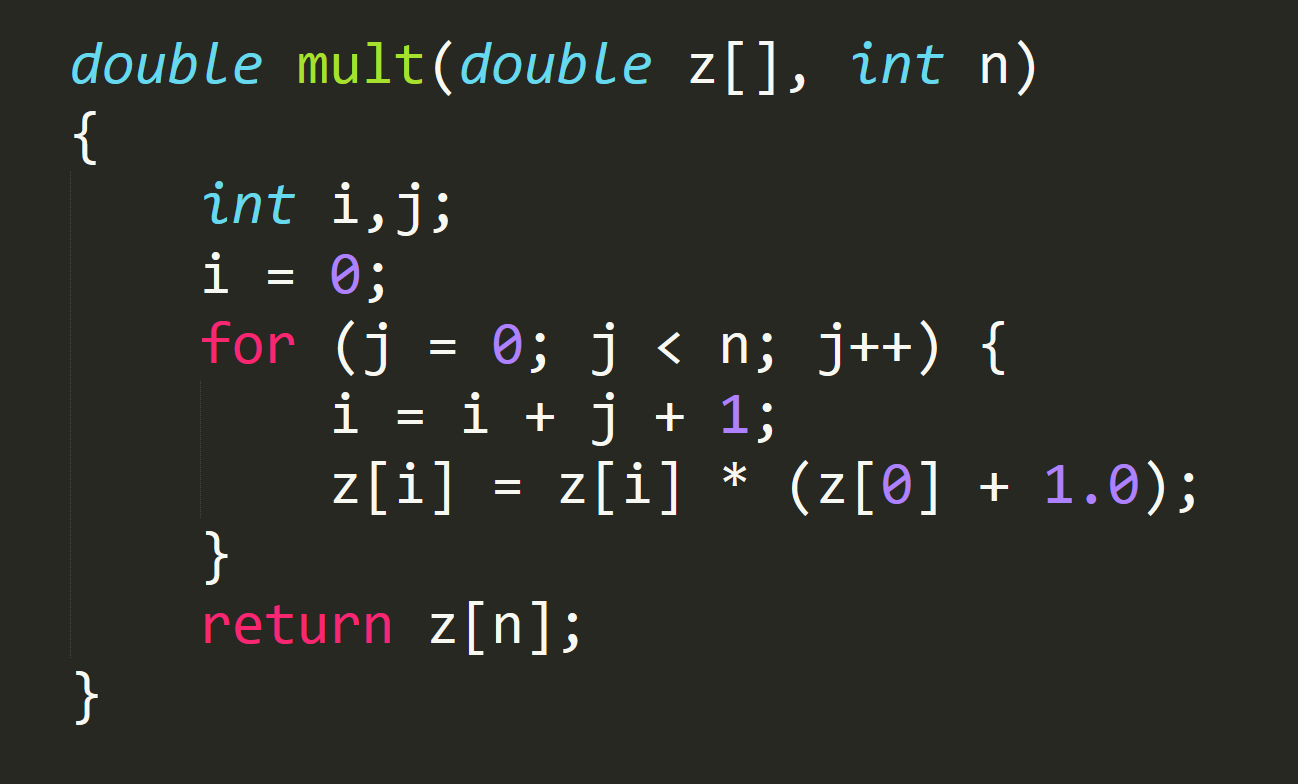
\includegraphics[width = .6\textwidth]{../figures/failC.PNG}
	\end{figure}
	
\end{frame}

\begin{frame}{How \ddp\ finds the minimal set of C tokens that causes the crash}
	\begin{tabular}{c l c}
				\hashtag & GCC input & test \\
				\hline
				1 & double mult($\dots$) $\{ int \; i, j; \; i = 0; \; for (\dots) \{ \dots\} \dots\}$ & $\xmark$ \\
				2 &\gray{ double mult($\dots$) $\{ int \; i, j; \; i = 0; \; for (\dots) \{ \dots\} \dots\}$} & $\cmark$ \\
				3 & double mult($\dots$) $\{\gray{ int \; i, j; \; i = 0; \; for (\dots) \{ \dots\} \dots}\}$ & $\cmark$ \\
				4 & double mult($\dots$) $\{ int \; i, j; \; i = 0; \; \gray{for (\dots) \{ \dots\} \dots}\}$ & $\cmark$ \\
				5 & double mult($\dots$) $\{ int \; i, j; \; i = 0; \; for (\dots) \{ \dots\}\gray{ \dots}\}$ & $\xmark$ \\
				6 & double mult($\dots$) $\{ int \; i, j; \; i = 0; \; for (\gray{\dots}) \{ \dots\} \gray{\dots}\}$ & $\cmark$ \\

				\vdots & \multicolumn{1}{c}{\vdots} & \vdots \\
				18 & \multicolumn{1}{c}{\dots \quad $z[i] = z[i] * (z[0] + 1.0);$ \quad \dots } & \xmark \\
				19 & \multicolumn{1}{c}{\dots \quad $z[i] = z[i] * (z[0] \gray{+ 1.0});$ \quad \dots } & \cmark \\
				20 & \multicolumn{1}{c}{\dots \quad $z[i] = z[i] * (z[0] \gray{+} 1.0);$ \quad \dots } & \qmark \\
				21 & \multicolumn{1}{c}{\dots \quad $z[i] = z[i] * (z[0] + \gray{1.0});$ \quad \dots } & \qmark \\
		\end{tabular}

\end{frame}